%%%%%%%%%%%%%%%%%%%%%%%%%%%%%%%%%%%%%%%%%
% Beamer Presentation
% LaTeX Template
% Version 1.0 (10/11/12)
%
% This template has been downloaded from:
% http://www.LaTeXTemplates.com
%
% License:
% CC BY-NC-SA 3.0 (http://creativecommons.org/licenses/by-nc-sa/3.0/)
%
%%%%%%%%%%%%%%%%%%%%%%%%%%%%%%%%%%%%%%%%%

%----------------------------------------------------------------------------------------
%	PACKAGES AND THEMES
%----------------------------------------------------------------------------------------

\documentclass{beamer}

\mode<presentation> {

% The Beamer class comes with a number of default slide themes
% which change the colors and layouts of slides. Below this is a list
% of all the themes, uncomment each in turn to see what they look like.

%\usetheme{default}
%\usetheme{AnnArbor}
%\usetheme{Antibes}
%\usetheme{Bergen}
%\usetheme{Berkeley}
%\usetheme{Berlin}
%\usetheme{Boadilla}
%\usetheme{CambridgeUS}
%\usetheme{Copenhagen}
%\usetheme{Darmstadt}
%\usetheme{Dresden}
%\usetheme{Frankfurt}
%\usetheme{Goettingen}
%\usetheme{Hannover}
%\usetheme{Ilmenau}
%\usetheme{JuanLesPins}
%\usetheme{Luebeck}
\usetheme{Madrid}
%\usetheme{Malmoe}
%\usetheme{Marburg}
%\usetheme{Montpellier}
%\usetheme{PaloAlto}
%\usetheme{Pittsburgh}
%\usetheme{Rochester}
%\usetheme{Singapore}
%\usetheme{Szeged}
%\usetheme{Warsaw}

% As well as themes, the Beamer class has a number of color themes
% for any slide theme. Uncomment each of these in turn to see how it
% changes the colors of your current slide theme.

%\usecolortheme{albatross}
%\usecolortheme{beaver}
%\usecolortheme{beetle}
%\usecolortheme{crane}
%\usecolortheme{dolphin}
%\usecolortheme{dove}
%\usecolortheme{fly}
%\usecolortheme{lily}
%\usecolortheme{orchid}
%\usecolortheme{rose}
%\usecolortheme{seagull}
\usecolortheme{seahorse}
%\usecolortheme{whale}
%\usecolortheme{wolverine}

%\setbeamertemplate{footline} % To remove the footer line in all slides uncomment this line
%\setbeamertemplate{footline}[page number] % To replace the footer line in all slides with a simple slide count uncomment this line

%\setbeamertemplate{navigation symbols}{} % To remove the navigation symbols from the bottom of all slides uncomment this line
}

\usepackage{graphicx} % Allows including images
\DeclareGraphicsExtensions{.pdf,.png,.jpg}
\usepackage{booktabs} % Allows the use of \toprule, \midrule and \bottomrule in tables
\usepackage[skip = 2pt, font=scriptsize]{caption}
\usepackage{subcaption}
%\usepackage{subfigure}

%----------------------------------------------------------------------------------------
%	TITLE PAGE
%----------------------------------------------------------------------------------------

\title[$B^0$ $\rightarrow$ $K^{*0}$ $\mu$ $\mu$]{LHCb MC group meeting: $B^0$ $\rightarrow$ $K^{*0}$ $\mu$ $\mu$} % The short title appears at the bottom of every slide, the full title is only on the title page

\author{Oliver Dahme} % Your name
\institute[UZH] % Your institution as it will appear on the bottom of every slide, may be shorthand to save space
{
University of Zurich \\ % Your institution for the title page
\medskip
\textit{o.dahme@cern.ch} % Your email address
}
\date{\today} % Date, can be changed to a custom date

\begin{document}

\begin{frame}
\titlepage % Print the title page as the first slide
\end{frame}

%\begin{frame}
%\frametitle{Overview} % Table of contents slide, comment this block out to remove it
%\tableofcontents % Throughout your presentation, if you choose to use \section{} and \subsection{} commands, these will automatically be printed on this slide as an overview of your presentation
%\end{frame}

%----------------------------------------------------------------------------------------
%	PRESENTATION SLIDES
%----------------------------------------------------------------------------------------

% all ten roc curves, btd histogram
% look at correlation at 20% 40% etc. bdt cut.

%------------------------------------------------
\section{Introduction} % Sections can be created in order to organize your presentation into discrete blocks, all sections and subsections are automatically printed in the table of contents as an overview of the talk
%------------------------------------------------

\begin{frame}
\frametitle{$B^0$ $\rightarrow$ $K^{*0}$ $\mu$ $\mu$}

\begin{itemize}
  \item Decay is a FCNC
  \item four charged particles in final state:
  \item $K^+$ and $\pi^-$ from the $K^{*0}$ decay
  \item two leptons from loop or box diagrams:
\end{itemize}


\begin{figure}
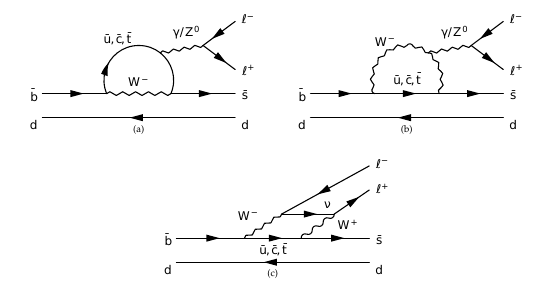
\includegraphics[width=0.8\linewidth]{KstarFeynman}
\caption{Feynman diagrams for decay $B_d$ $\rightarrow$ $\mu^+$ $\mu^-$ at lowest order}
\end{figure}
\end{frame}

\begin{frame}
\frametitle{$B^0$ $\rightarrow$ $K^{*0}$ $\mu$ $\mu$}
three angels define the kinematics of the decay:
\begin{itemize}
  \item ThetaK or $\theta_K$
  \item ThetaL or $\theta_L$
  \item Phi or $\phi$
\end{itemize}

\begin{figure}
  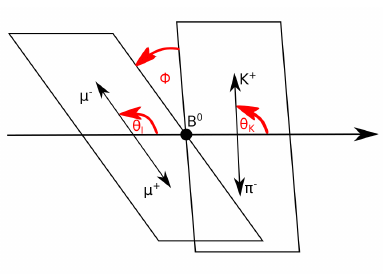
\includegraphics[width=0.6\linewidth]{angels}
  \caption{kinematic variables of the decay $B^0$ $\rightarrow$ $K^{*0}$ $\mu$ $\mu$}
\end{figure}

\end{frame}


\begin{frame}
  \frametitle{classification with Machine Learning (BDT)}
  \begin{itemize}
    \item to eliminate combinatorial background, Boost Decision Trees are used as a black box to classify data into signal and background.
    \item They assign a 'probability' to each event
    \item sk bdt from the scikit-learn package is used, and uBoost from the hep ml package
    \item average of both gives the BDT response
    \item training has been performed on the Linux Cluster in Zurich
  \end{itemize}
\end{frame}

\begin{frame}
  \frametitle{Region to train}
  \begin{itemize}
    \item you want the bdt to train in the background region
    \item J/Psi has two resonance which will be cut off
  \end{itemize}

  \begin{figure}
\centering
\begin{subfigure}{0.5\textwidth}
  \centering
  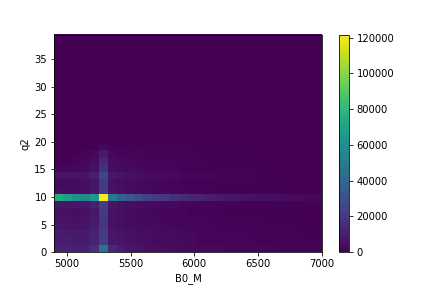
\includegraphics[width=1\linewidth]{beforeCutPlot}
  \caption{Before Cut}
\end{subfigure}%
\begin{subfigure}{0.5\textwidth}
  \centering
  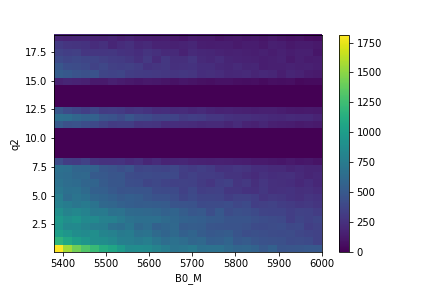
\includegraphics[width=1\linewidth]{cutPlot}
  \caption{After Cut}
\end{subfigure}
\end{figure}

\end{frame}

\begin{frame}
  \frametitle{training of the BDTs}
  8 train parameters:
  \begin{itemize}
    \item B0 P
    \item B0 PT
    \item B0 ENDVERTEX CHI2
    \item B0 IP OWNPV
    \item B0 IPCHI2 OWNPV
    \item B0 FD OWNPV
    \item B0 FDCHI2 OWNPV
    \item B0 relinfo VTXISOBDTHARDFIRSTVALUE
  \end{itemize}
  4 uniform parameters:
  \begin{itemize}
    \item B0 M
    \item B0 ThetaK
    \item B0 ThetaL
    \item B0 Phi
  \end{itemize}
  uniform parameters have to be uncorrelated since we know that from physics.
  But BDT might find a correlation which is bad.
\end{frame}

\begin{frame}
  \frametitle{BDT correlation check}

  \begin{figure}
  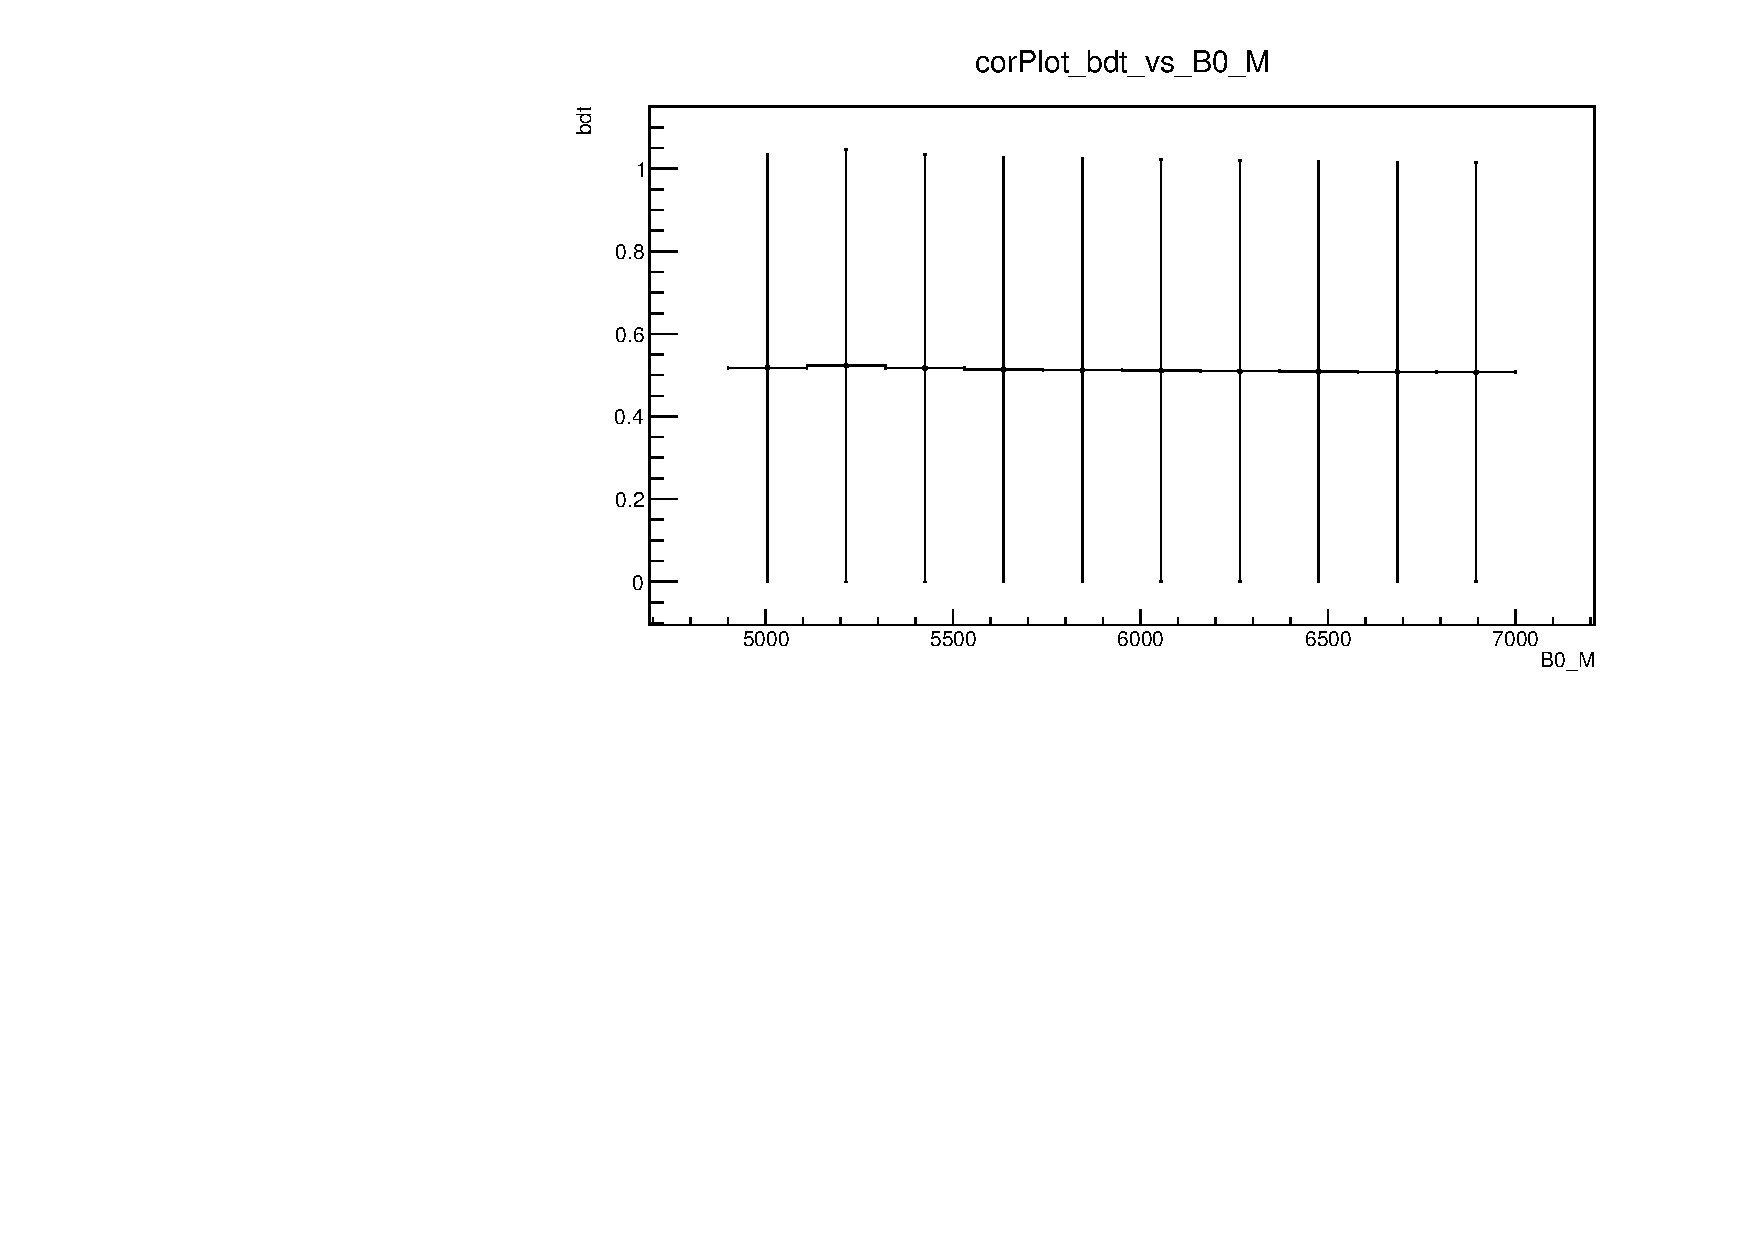
\includegraphics[width=1.0\linewidth]{plots/corPlot_bdt_vs_B0_M.pdf}
  \end{figure}

\end{frame}

\begin{frame}
  \frametitle{BDT correlation check}

  \begin{figure}
  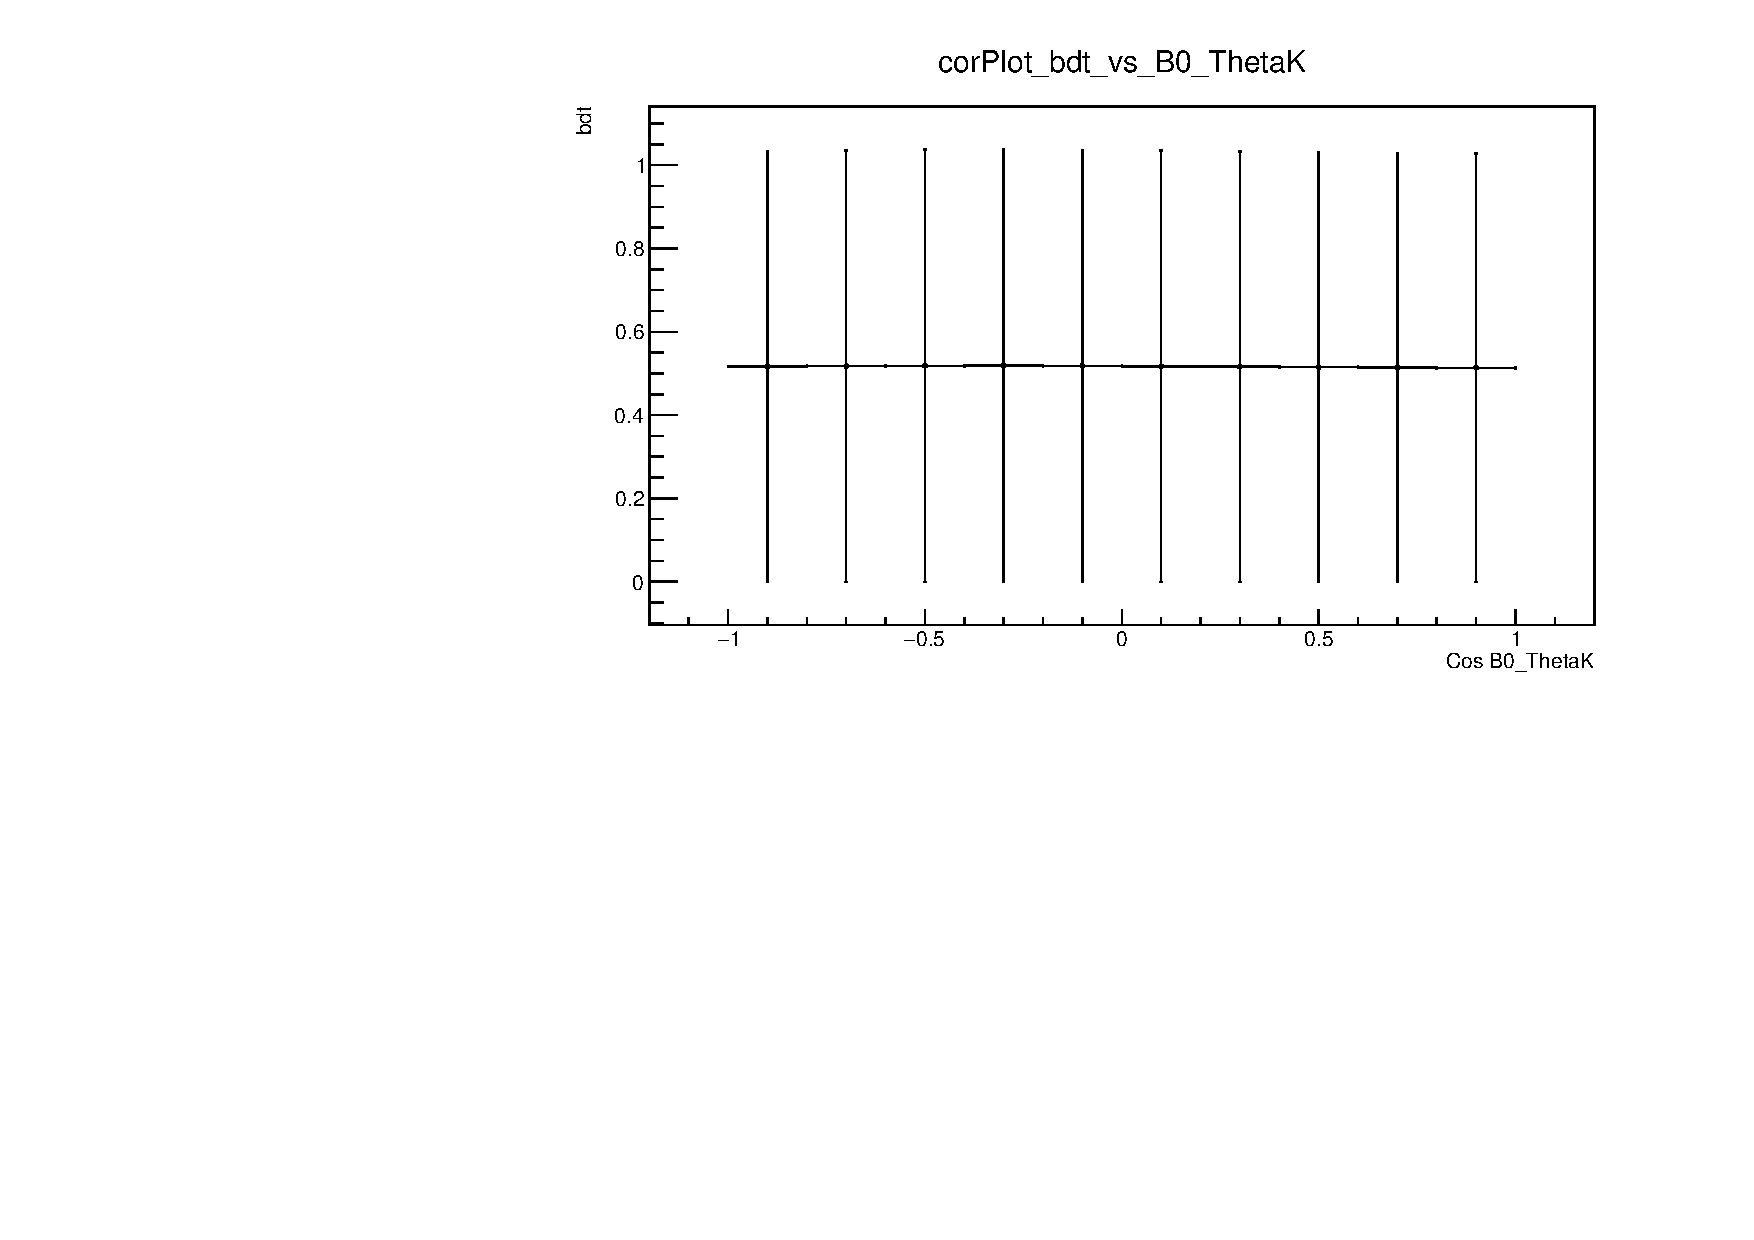
\includegraphics[width=1.0\linewidth]{plots/corPlot_bdt_vs_B0_ThetaK.pdf}
  \end{figure}

\end{frame}

\begin{frame}
  \frametitle{BDT correlation check}

  \begin{figure}
  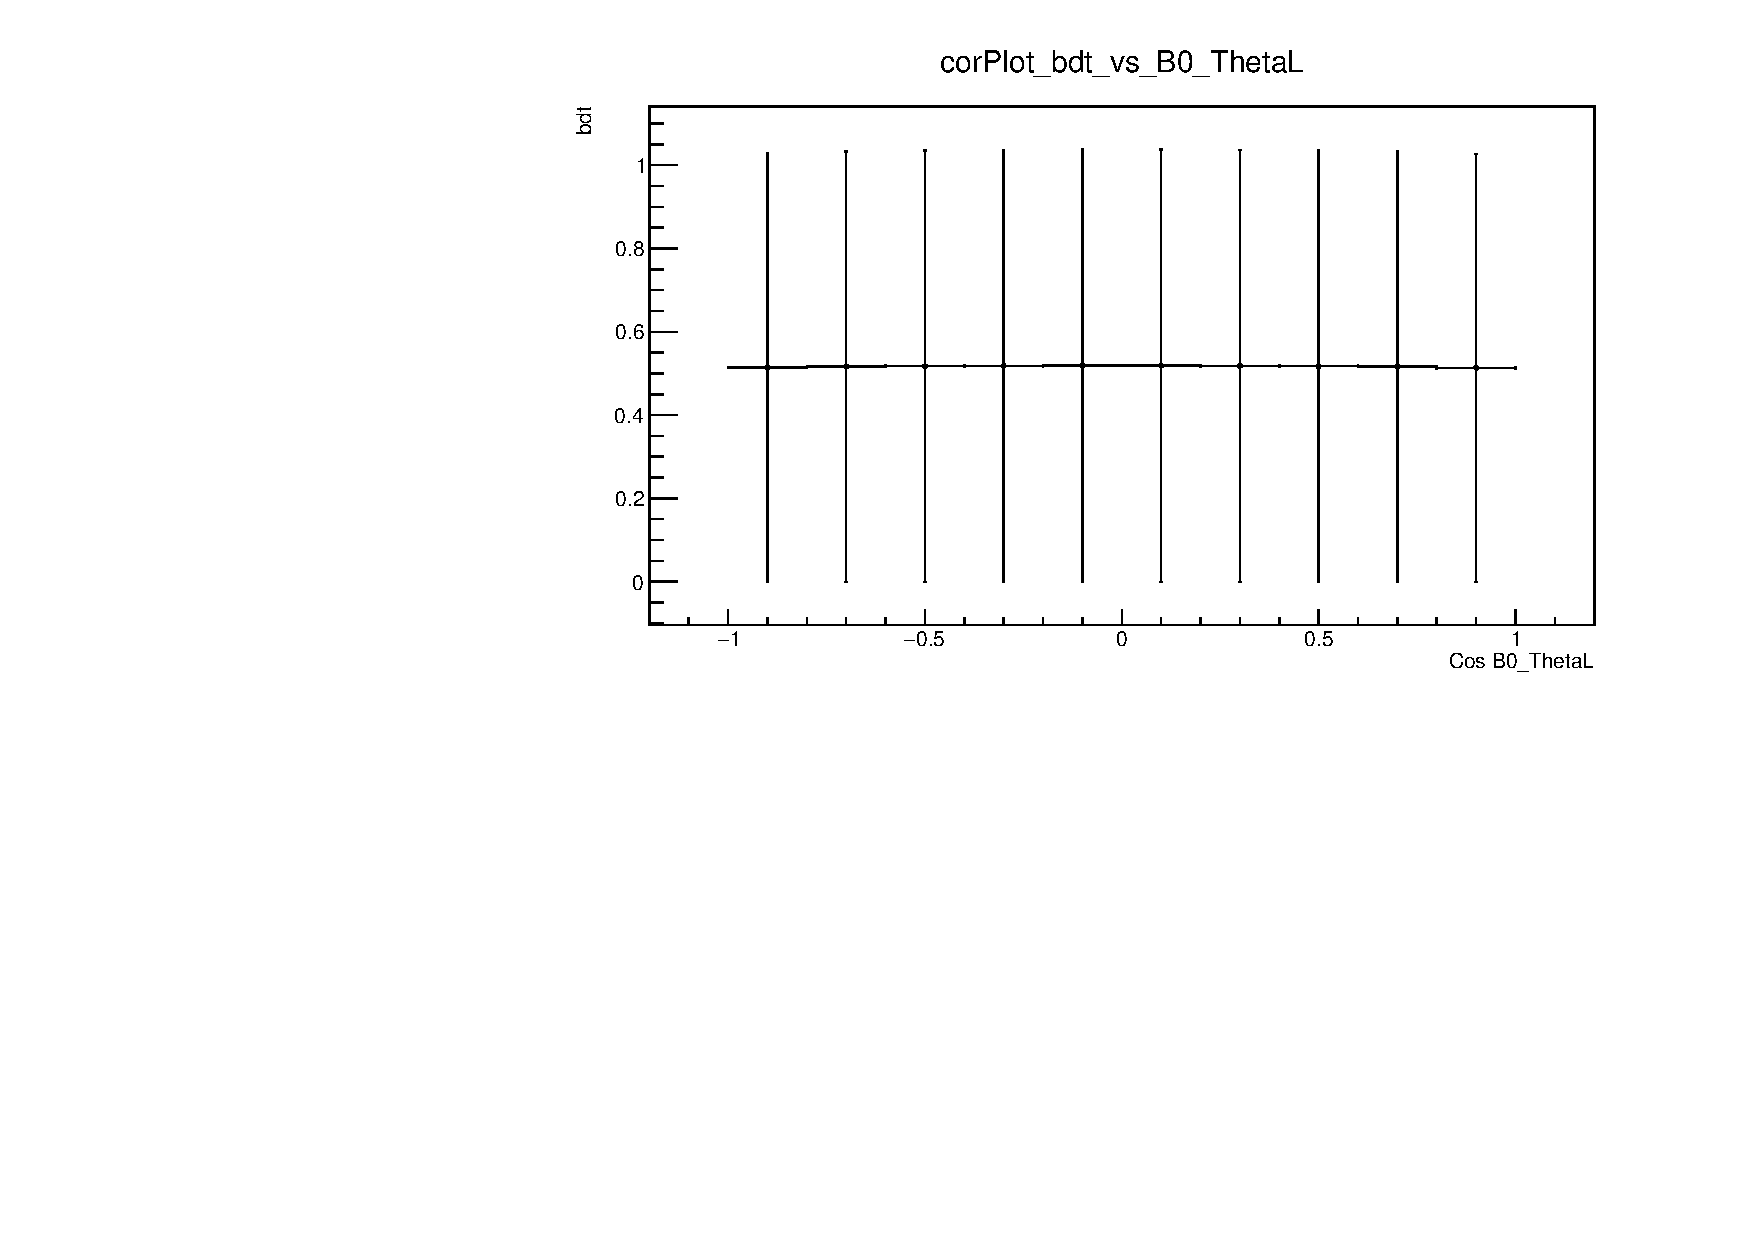
\includegraphics[width=1.0\linewidth]{plots/corPlot_bdt_vs_B0_ThetaL.pdf}
  \end{figure}

\end{frame}

\begin{frame}
  \frametitle{BDT correlation check}

  \begin{figure}
  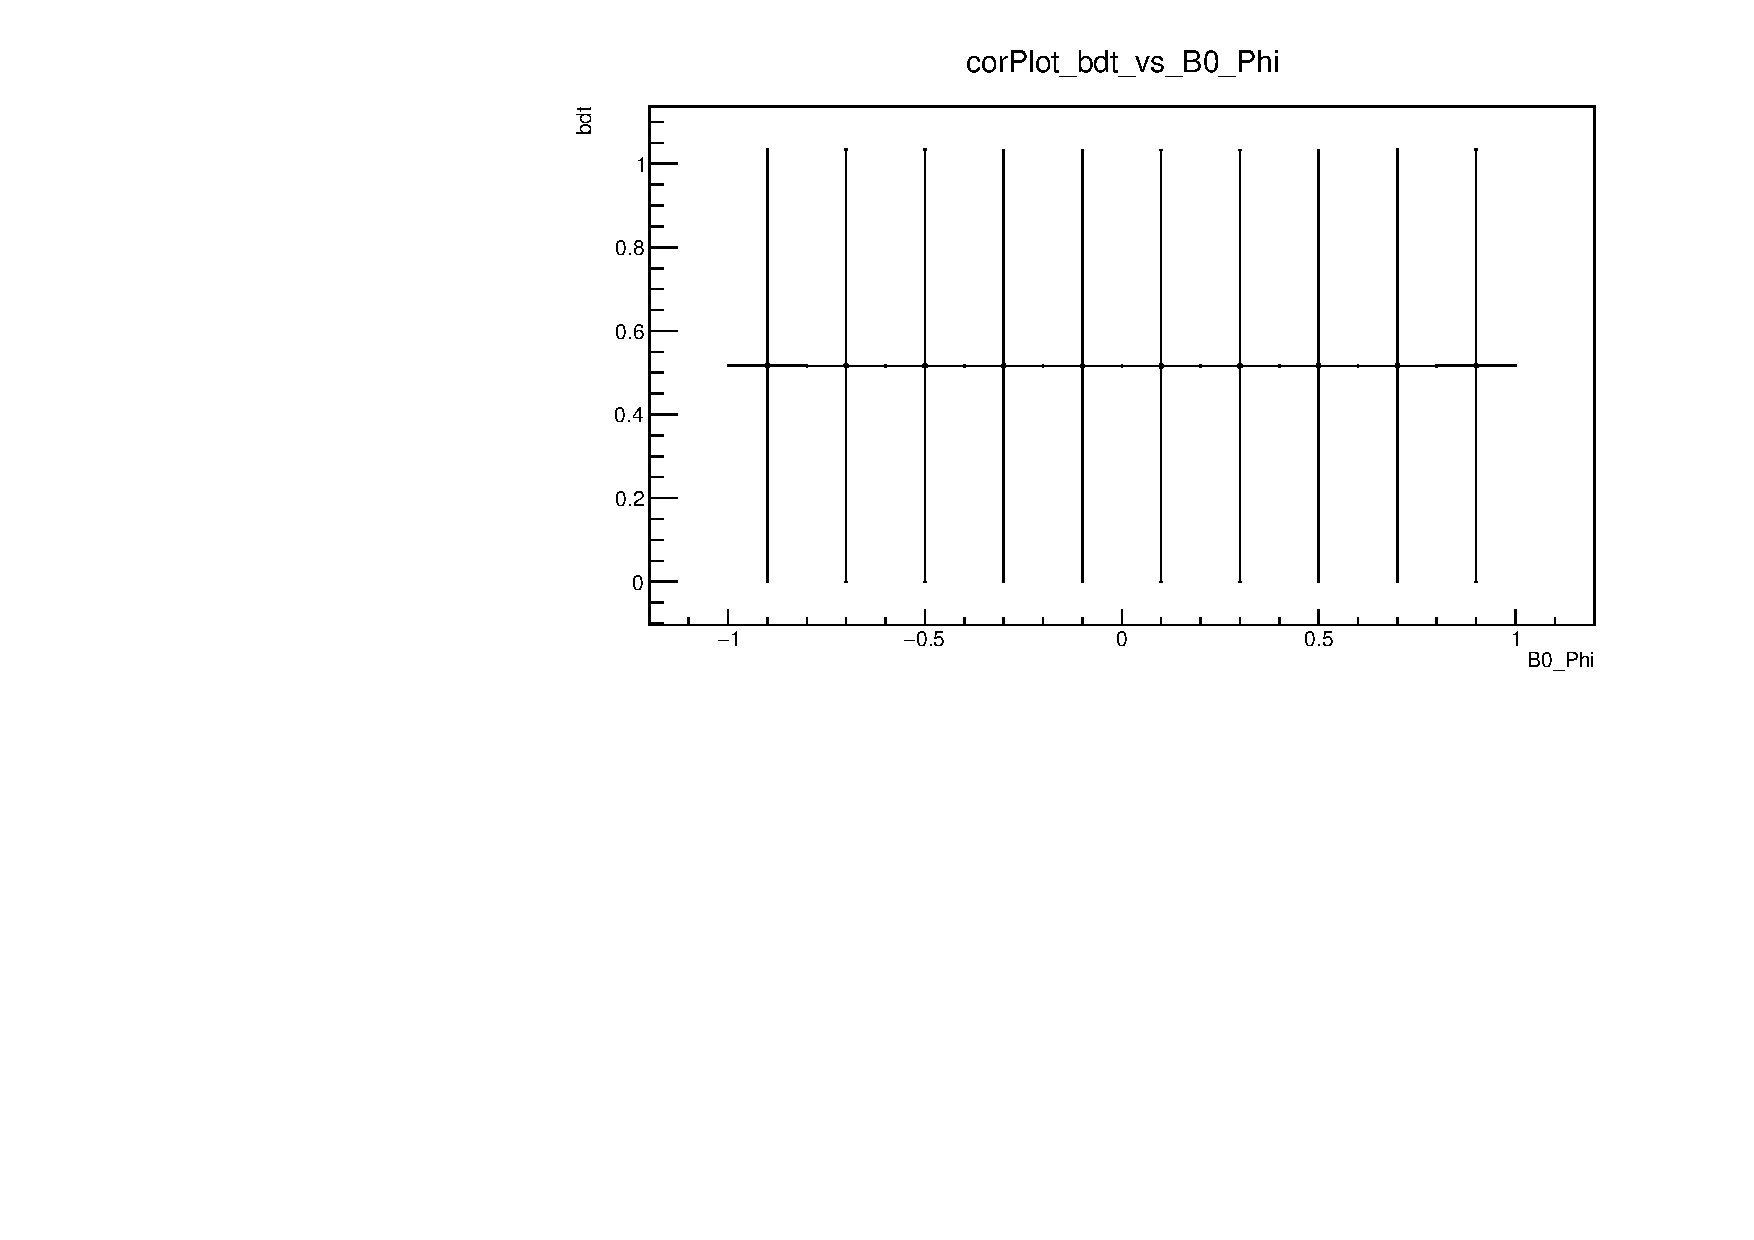
\includegraphics[width=1.0\linewidth]{plots/corPlot_bdt_vs_B0_Phi.pdf}
  \end{figure}

\end{frame}



%----------------------------------------------------------------------------------------



\end{document}
